\documentclass[11pt]{article}
\usepackage[textwidth=18.0cm, textheight=23.0cm, top=2.0cm]{geometry}
\usepackage{pst-all}
\usepackage{amssymb}
\usepackage{tikz}
\usepackage{underscore}\begin{document}
\pagestyle{empty}


ClassName: \underline{\textbf{Class_10.2bp-24}}
\par
BinSize: \underline{\textbf{100 × 100}}
\par
ReduceSize: \underline{\textbf{100 × 100}}
\par
TypeNum: \underline{\textbf{59}}
\par
Num: \underline{\textbf{60}}
\par
OutS: \underline{\textbf{80000}}
\par
InS: \underline{\textbf{72107}}
\par
Rate: \underline{\textbf{0.901}}
\par
UB: \underline{\textbf{8}}
\par
LB0: \underline{\textbf{8}}
\par
LB: \underline{\textbf{8}}
\par
LBWithCut: \underline{\textbf{8}}
\par
NodeCut: \underline{\textbf{0}}
\par
ExtendedNodeCnt: \underline{\textbf{1}}
\par
GenNodeCnt: \underline{\textbf{1}}
\par
PrimalNode: \underline{\textbf{0}}
\par
ColumnCount: \underline{\textbf{8}}
\par
TotalCutCount: \underline{\textbf{0}}
\par
RootCutCount: \underline{\textbf{0}}
\par
LPSolverCnt: \underline{\textbf{1}}
\par
PricingSolverCnt: \underline{\textbf{0}}
\par
BranchAndBoundNum: \underline{\textbf{1}}
\par
isOpt: \underline{\textbf{true}}
\par
TimeOnInitSolution: \underline{\textbf{0.030 s}}
\par
TimeOnPrimal: \underline{\textbf{0.000 s}}
\par
TimeOnPricing: \underline{\textbf{0.000 s}}
\par
TimeOnRmp: \underline{\textbf{0.078 s}}
\par
TotalTime: \underline{\textbf{0.171 s}}
\par
\newpage


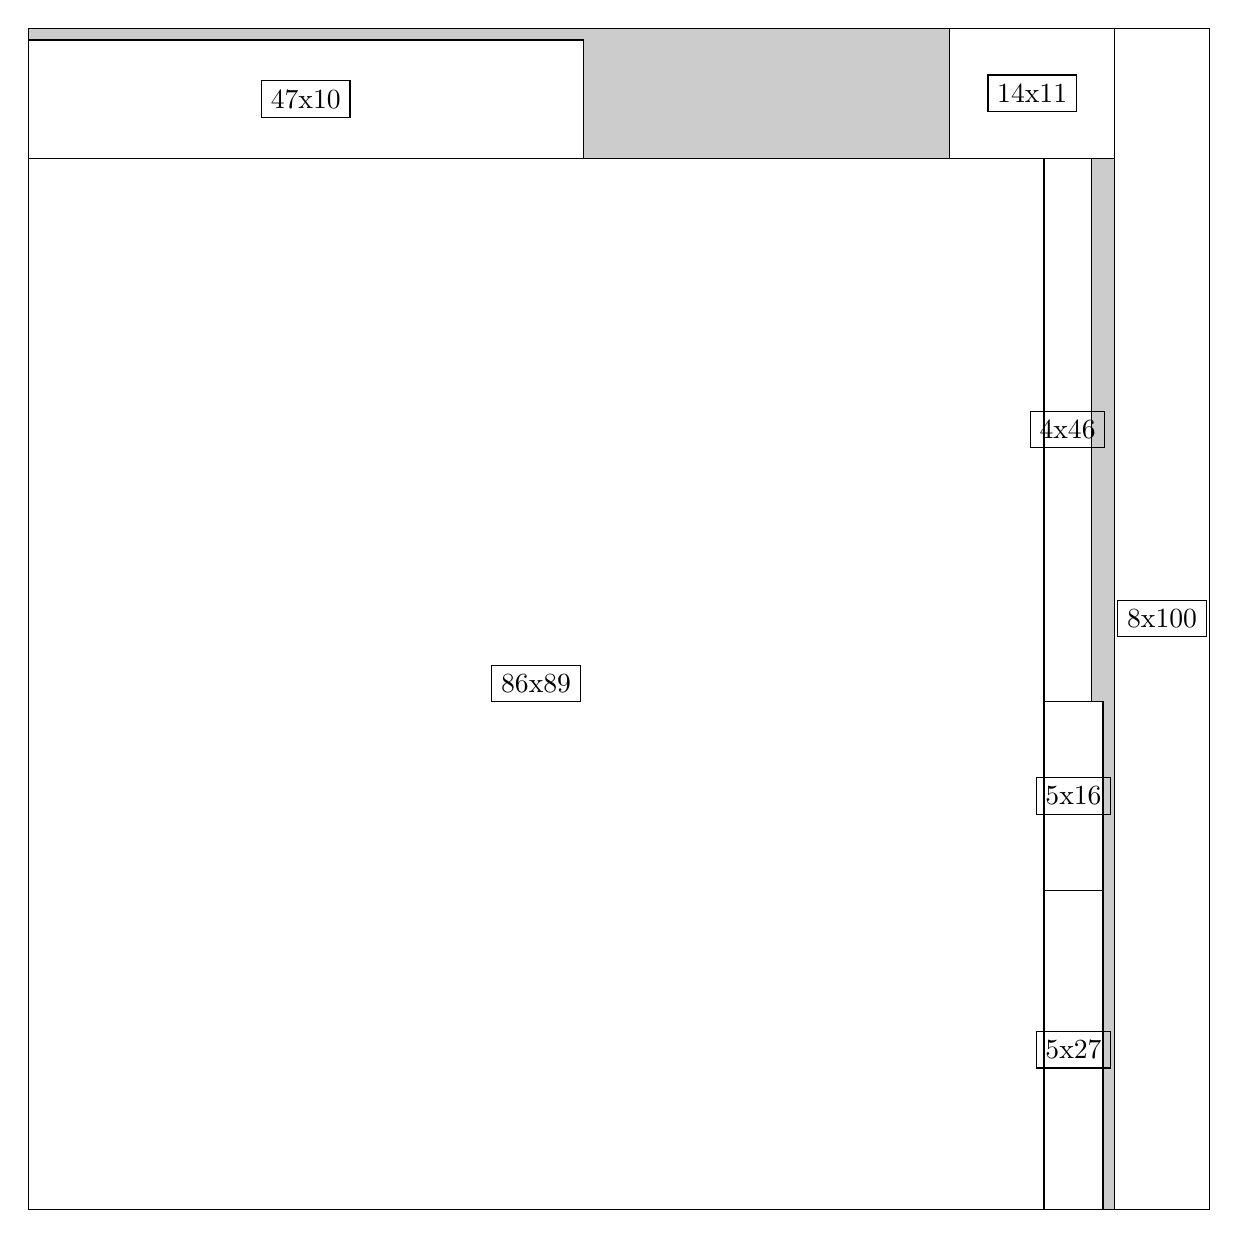
\begin{tikzpicture}[shorten >=1pt,scale=1.0,every node/.style={scale=1.0},->]
\tikzstyle{vertex}=[circle,fill=black!25,minimum size=14pt,inner sep=0pt]
\filldraw[fill=gray!40!white, draw=black] (0,0) rectangle (15.0,15.0);
\foreach \name/\x/\y/\w/\h in {86x89/0.0/0.0/12.9/13.35,5x27/12.9/0.0/0.75/4.05,8x100/13.799999999999999/0.0/1.2/15.0,47x10/0.0/13.35/7.05/1.5,4x46/12.9/6.45/0.6/6.8999999999999995,14x11/11.7/13.35/2.1/1.65,5x16/12.9/4.05/0.75/2.4}
\filldraw[fill=white!40!white, draw=black] (\x,\y) rectangle node[draw] (\name) {\name} ++(\w,\h);
\end{tikzpicture}


w =86 , h =89 , x =0 , y =0 , v =7654
\par
w =5 , h =27 , x =86 , y =0 , v =135
\par
w =8 , h =100 , x =92 , y =0 , v =800
\par
w =47 , h =10 , x =0 , y =89 , v =470
\par
w =4 , h =46 , x =86 , y =43 , v =184
\par
w =14 , h =11 , x =78 , y =89 , v =154
\par
w =5 , h =16 , x =86 , y =27 , v =80
\par
\newpage


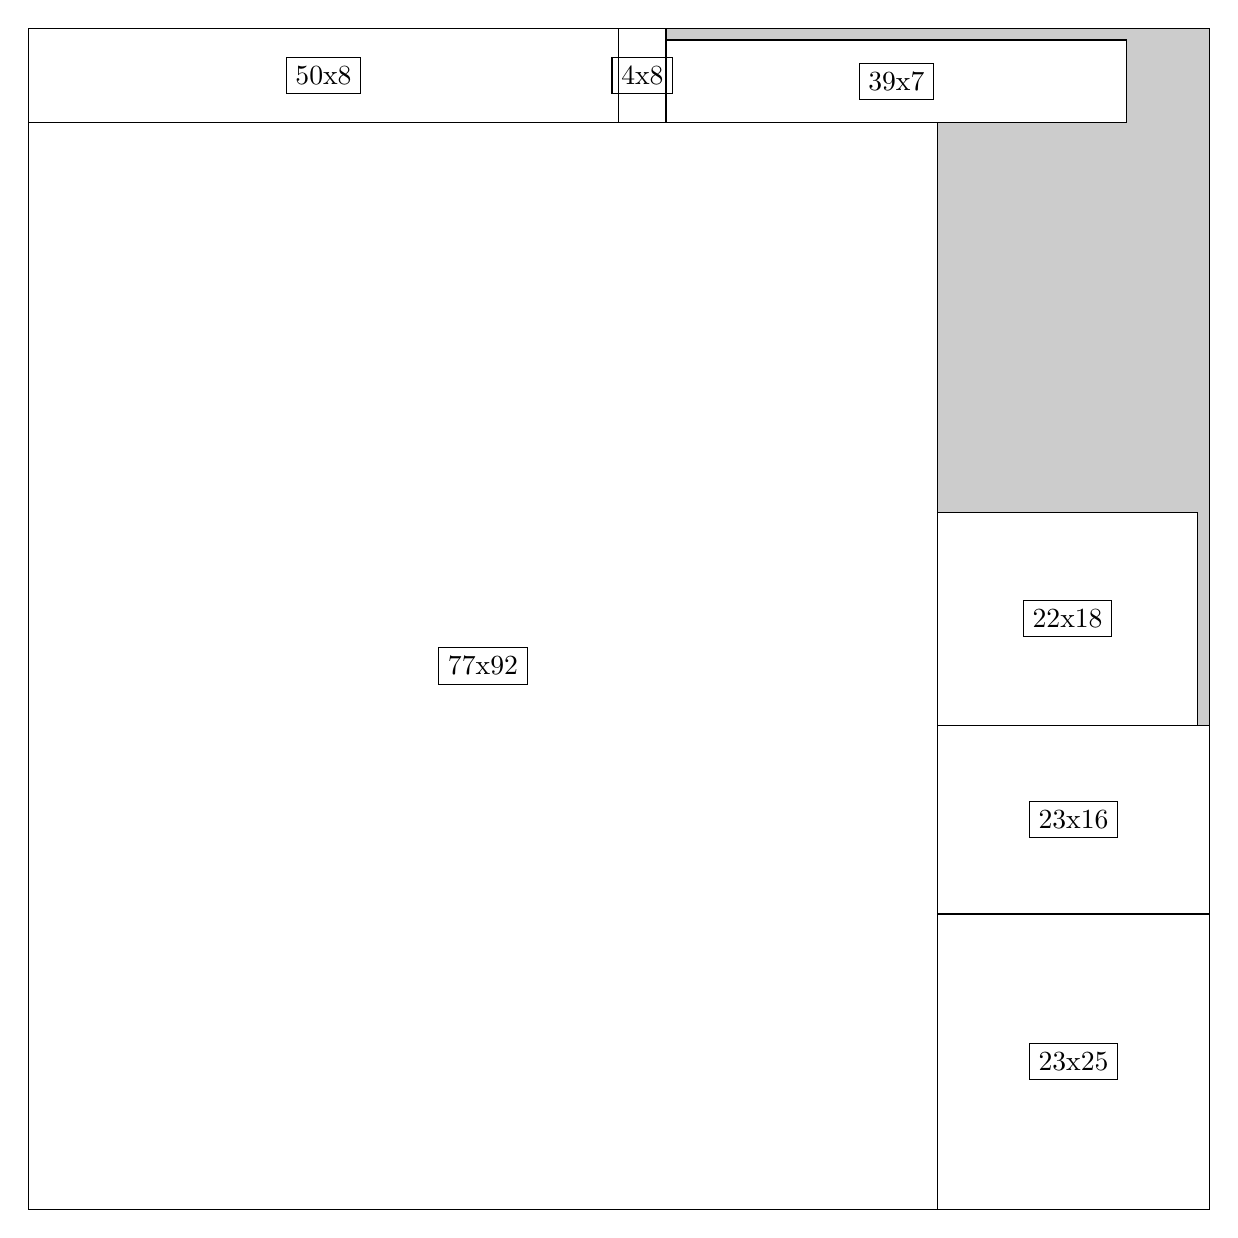
\begin{tikzpicture}[shorten >=1pt,scale=1.0,every node/.style={scale=1.0},->]
\tikzstyle{vertex}=[circle,fill=black!25,minimum size=14pt,inner sep=0pt]
\filldraw[fill=gray!40!white, draw=black] (0,0) rectangle (15.0,15.0);
\foreach \name/\x/\y/\w/\h in {77x92/0.0/0.0/11.549999999999999/13.799999999999999,23x25/11.549999999999999/0.0/3.4499999999999997/3.75,50x8/0.0/13.799999999999999/7.5/1.2,22x18/11.549999999999999/6.1499999999999995/3.3/2.6999999999999997,23x16/11.549999999999999/3.75/3.4499999999999997/2.4,39x7/8.1/13.799999999999999/5.85/1.05,4x8/7.5/13.799999999999999/0.6/1.2}
\filldraw[fill=white!40!white, draw=black] (\x,\y) rectangle node[draw] (\name) {\name} ++(\w,\h);
\end{tikzpicture}


w =77 , h =92 , x =0 , y =0 , v =7084
\par
w =23 , h =25 , x =77 , y =0 , v =575
\par
w =50 , h =8 , x =0 , y =92 , v =400
\par
w =22 , h =18 , x =77 , y =41 , v =396
\par
w =23 , h =16 , x =77 , y =25 , v =368
\par
w =39 , h =7 , x =54 , y =92 , v =273
\par
w =4 , h =8 , x =50 , y =92 , v =32
\par
\newpage


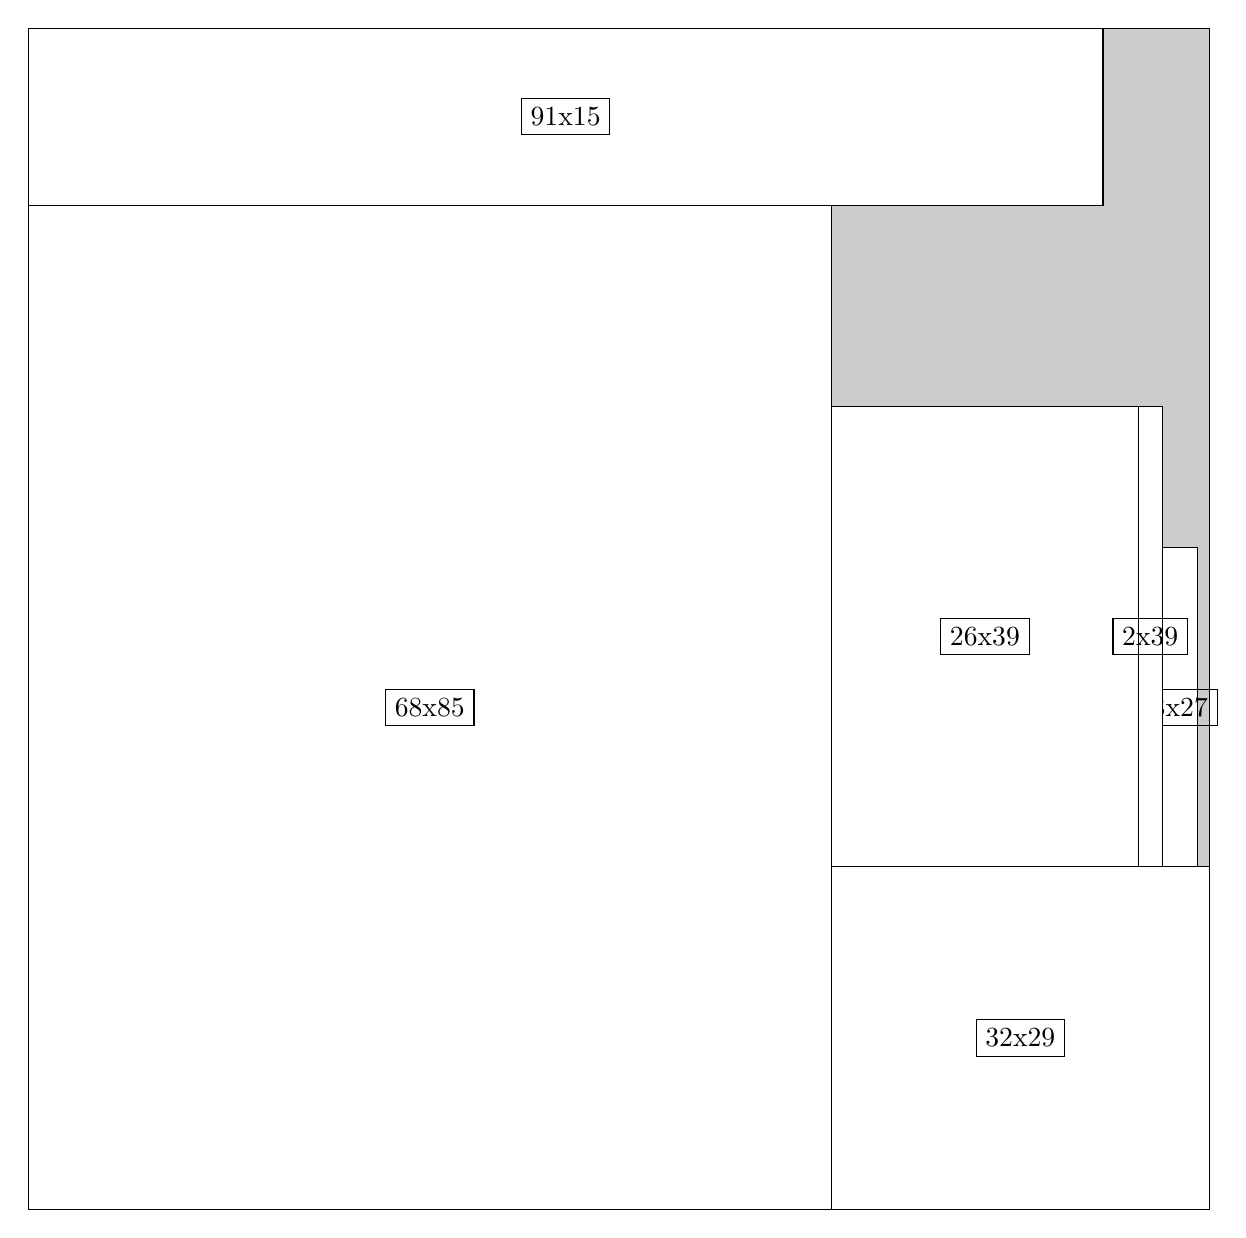
\begin{tikzpicture}[shorten >=1pt,scale=1.0,every node/.style={scale=1.0},->]
\tikzstyle{vertex}=[circle,fill=black!25,minimum size=14pt,inner sep=0pt]
\filldraw[fill=gray!40!white, draw=black] (0,0) rectangle (15.0,15.0);
\foreach \name/\x/\y/\w/\h in {68x85/0.0/0.0/10.2/12.75,91x15/0.0/12.75/13.65/2.25,26x39/10.2/4.35/3.9/5.85,32x29/10.2/0.0/4.8/4.35,3x27/14.399999999999999/4.35/0.44999999999999996/4.05,2x39/14.1/4.35/0.3/5.85}
\filldraw[fill=white!40!white, draw=black] (\x,\y) rectangle node[draw] (\name) {\name} ++(\w,\h);
\end{tikzpicture}


w =68 , h =85 , x =0 , y =0 , v =5780
\par
w =91 , h =15 , x =0 , y =85 , v =1365
\par
w =26 , h =39 , x =68 , y =29 , v =1014
\par
w =32 , h =29 , x =68 , y =0 , v =928
\par
w =3 , h =27 , x =96 , y =29 , v =81
\par
w =2 , h =39 , x =94 , y =29 , v =78
\par
\newpage


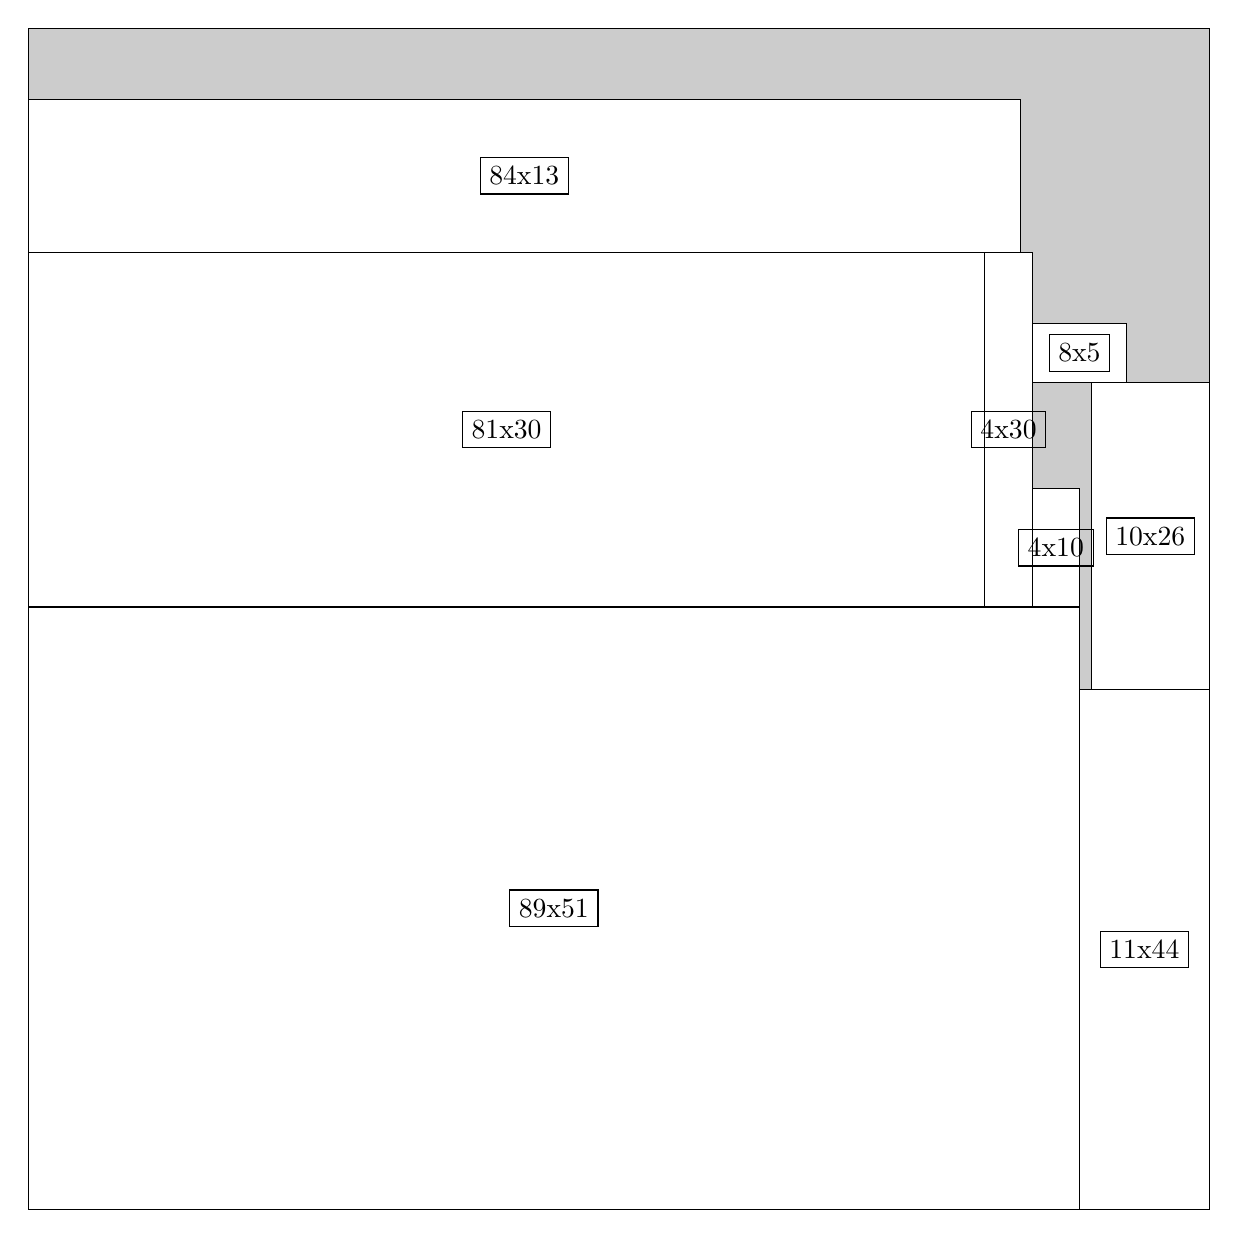
\begin{tikzpicture}[shorten >=1pt,scale=1.0,every node/.style={scale=1.0},->]
\tikzstyle{vertex}=[circle,fill=black!25,minimum size=14pt,inner sep=0pt]
\filldraw[fill=gray!40!white, draw=black] (0,0) rectangle (15.0,15.0);
\foreach \name/\x/\y/\w/\h in {89x51/0.0/0.0/13.35/7.6499999999999995,81x30/0.0/7.6499999999999995/12.15/4.5,84x13/0.0/12.15/12.6/1.95,11x44/13.35/0.0/1.65/6.6,10x26/13.5/6.6/1.5/3.9,4x30/12.15/7.6499999999999995/0.6/4.5,8x5/12.75/10.5/1.2/0.75,4x10/12.75/7.6499999999999995/0.6/1.5}
\filldraw[fill=white!40!white, draw=black] (\x,\y) rectangle node[draw] (\name) {\name} ++(\w,\h);
\end{tikzpicture}


w =89 , h =51 , x =0 , y =0 , v =4539
\par
w =81 , h =30 , x =0 , y =51 , v =2430
\par
w =84 , h =13 , x =0 , y =81 , v =1092
\par
w =11 , h =44 , x =89 , y =0 , v =484
\par
w =10 , h =26 , x =90 , y =44 , v =260
\par
w =4 , h =30 , x =81 , y =51 , v =120
\par
w =8 , h =5 , x =85 , y =70 , v =40
\par
w =4 , h =10 , x =85 , y =51 , v =40
\par
\newpage


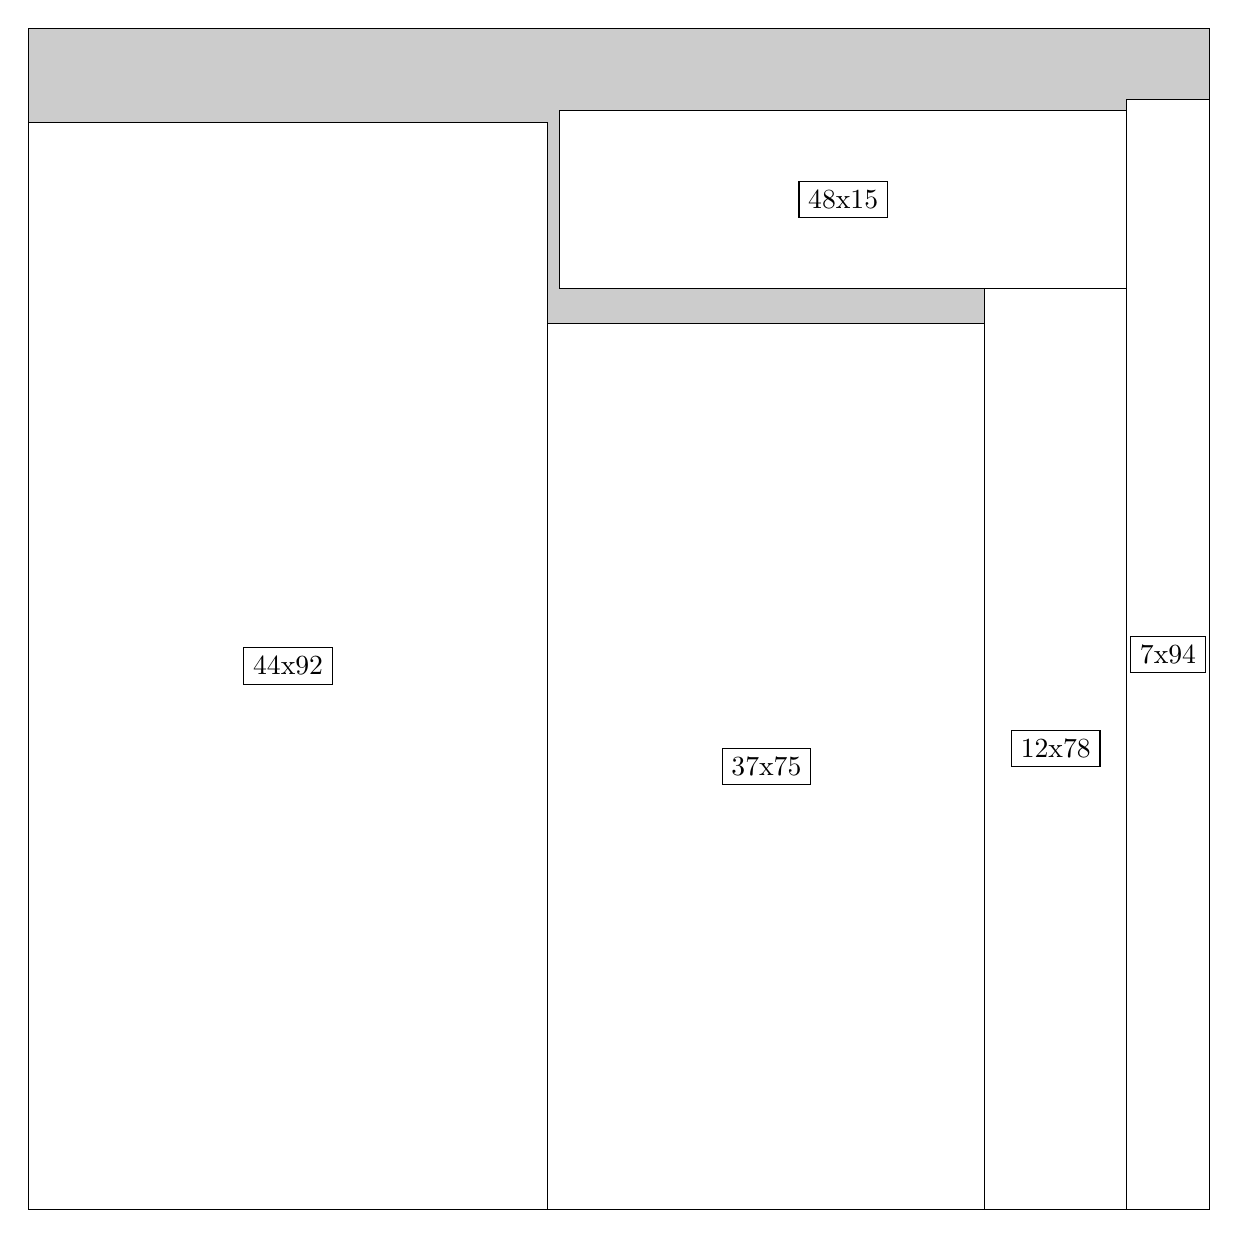
\begin{tikzpicture}[shorten >=1pt,scale=1.0,every node/.style={scale=1.0},->]
\tikzstyle{vertex}=[circle,fill=black!25,minimum size=14pt,inner sep=0pt]
\filldraw[fill=gray!40!white, draw=black] (0,0) rectangle (15.0,15.0);
\foreach \name/\x/\y/\w/\h in {44x92/0.0/0.0/6.6/13.799999999999999,37x75/6.6/0.0/5.55/11.25,12x78/12.15/0.0/1.7999999999999998/11.7,48x15/6.75/11.7/7.199999999999999/2.25,7x94/13.95/0.0/1.05/14.1}
\filldraw[fill=white!40!white, draw=black] (\x,\y) rectangle node[draw] (\name) {\name} ++(\w,\h);
\end{tikzpicture}


w =44 , h =92 , x =0 , y =0 , v =4048
\par
w =37 , h =75 , x =44 , y =0 , v =2775
\par
w =12 , h =78 , x =81 , y =0 , v =936
\par
w =48 , h =15 , x =45 , y =78 , v =720
\par
w =7 , h =94 , x =93 , y =0 , v =658
\par
\newpage


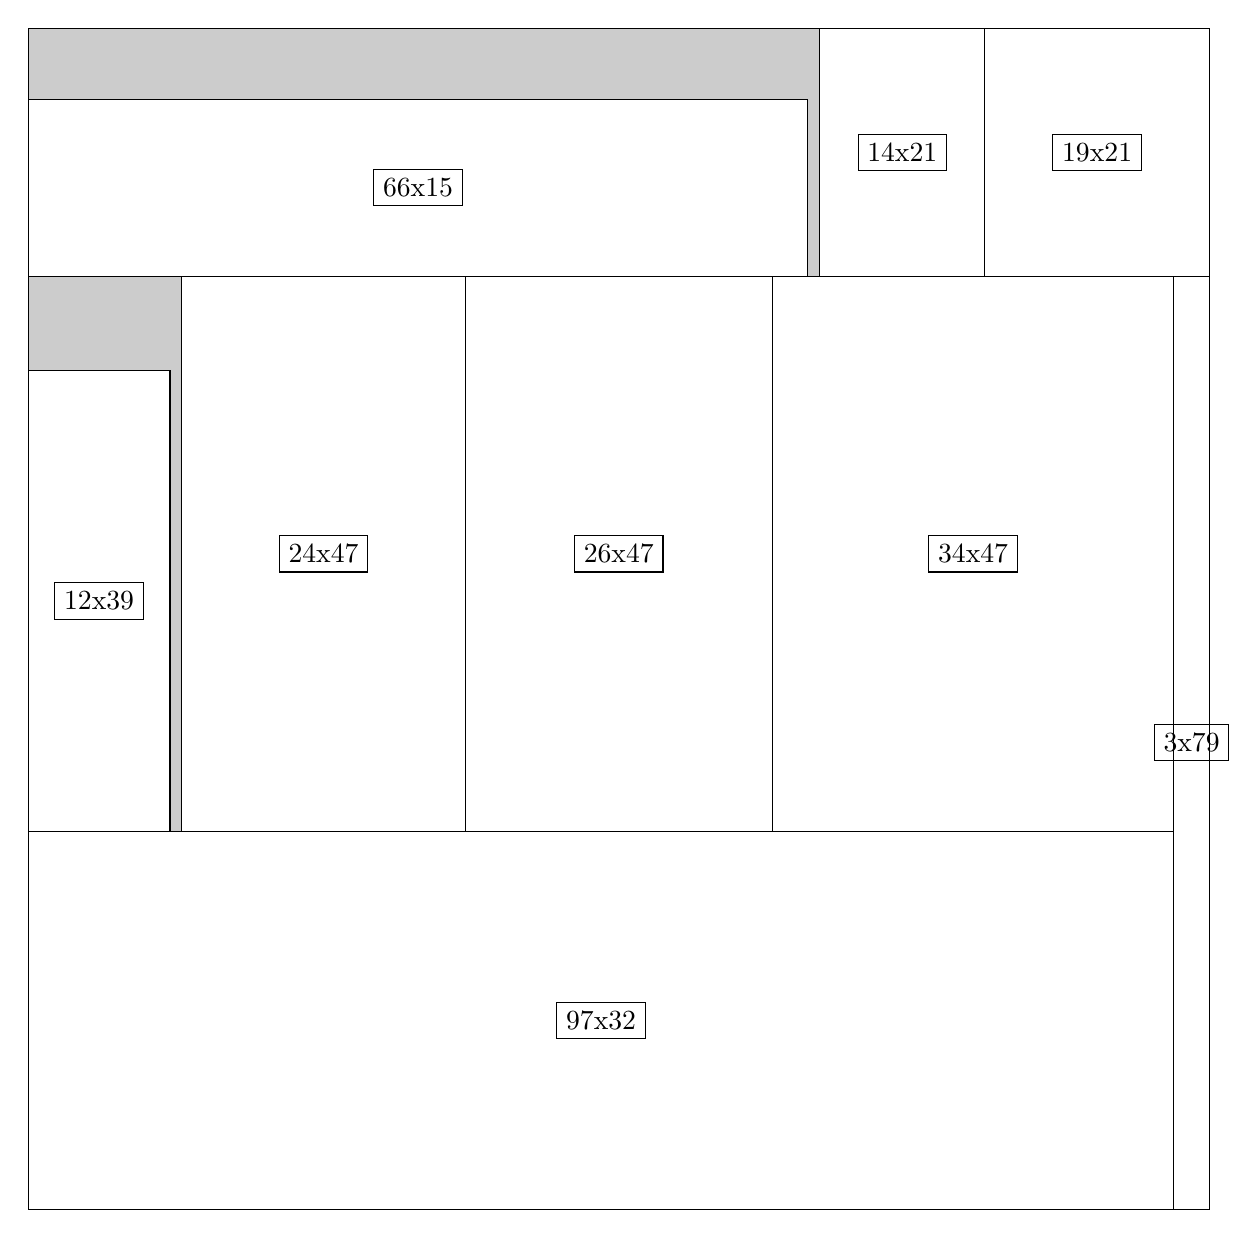
\begin{tikzpicture}[shorten >=1pt,scale=1.0,every node/.style={scale=1.0},->]
\tikzstyle{vertex}=[circle,fill=black!25,minimum size=14pt,inner sep=0pt]
\filldraw[fill=gray!40!white, draw=black] (0,0) rectangle (15.0,15.0);
\foreach \name/\x/\y/\w/\h in {97x32/0.0/0.0/14.549999999999999/4.8,34x47/9.45/4.8/5.1/7.05,26x47/5.55/4.8/3.9/7.05,66x15/0.0/11.85/9.9/2.25,12x39/0.0/4.8/1.7999999999999998/5.85,19x21/12.15/11.85/2.85/3.15,14x21/10.049999999999999/11.85/2.1/3.15,3x79/14.549999999999999/0.0/0.44999999999999996/11.85,24x47/1.95/4.8/3.5999999999999996/7.05}
\filldraw[fill=white!40!white, draw=black] (\x,\y) rectangle node[draw] (\name) {\name} ++(\w,\h);
\end{tikzpicture}


w =97 , h =32 , x =0 , y =0 , v =3104
\par
w =34 , h =47 , x =63 , y =32 , v =1598
\par
w =26 , h =47 , x =37 , y =32 , v =1222
\par
w =66 , h =15 , x =0 , y =79 , v =990
\par
w =12 , h =39 , x =0 , y =32 , v =468
\par
w =19 , h =21 , x =81 , y =79 , v =399
\par
w =14 , h =21 , x =67 , y =79 , v =294
\par
w =3 , h =79 , x =97 , y =0 , v =237
\par
w =24 , h =47 , x =13 , y =32 , v =1128
\par
\newpage


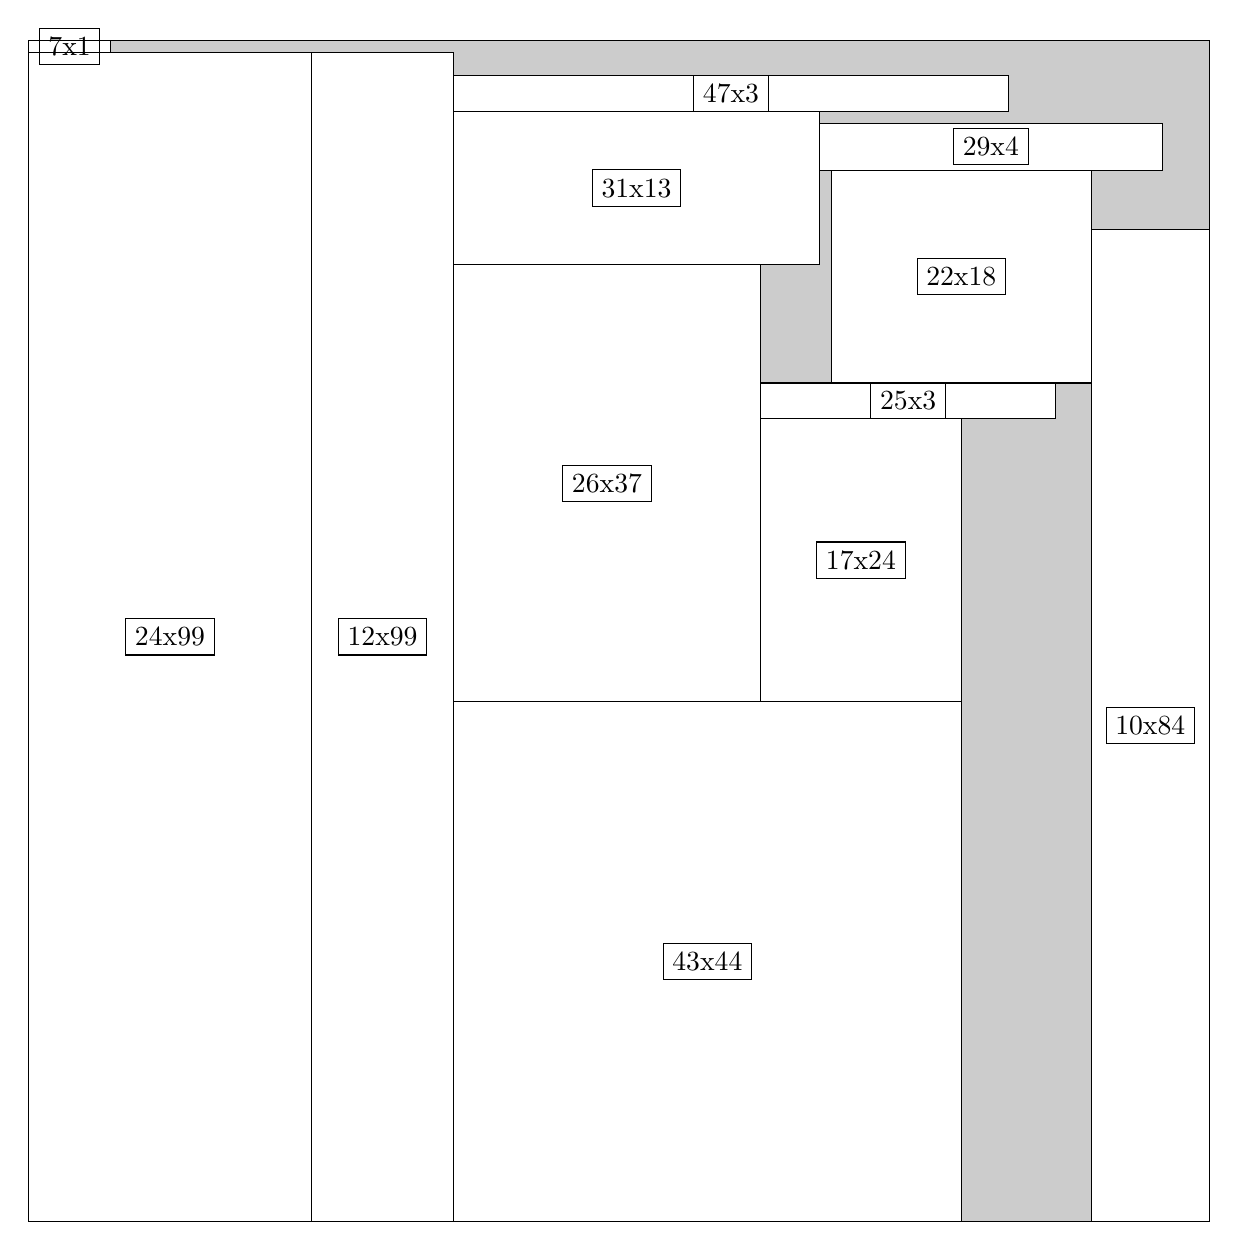
\begin{tikzpicture}[shorten >=1pt,scale=1.0,every node/.style={scale=1.0},->]
\tikzstyle{vertex}=[circle,fill=black!25,minimum size=14pt,inner sep=0pt]
\filldraw[fill=gray!40!white, draw=black] (0,0) rectangle (15.0,15.0);
\foreach \name/\x/\y/\w/\h in {24x99/0.0/0.0/3.5999999999999996/14.85,43x44/5.3999999999999995/0.0/6.45/6.6,12x99/3.5999999999999996/0.0/1.7999999999999998/14.85,26x37/5.3999999999999995/6.6/3.9/5.55,10x84/13.5/0.0/1.5/12.6,17x24/9.299999999999999/6.6/2.55/3.5999999999999996,31x13/5.3999999999999995/12.15/4.6499999999999995/1.95,22x18/10.2/10.65/3.3/2.6999999999999997,47x3/5.3999999999999995/14.1/7.05/0.44999999999999996,29x4/10.049999999999999/13.35/4.35/0.6,25x3/9.299999999999999/10.2/3.75/0.44999999999999996,7x1/0.0/14.85/1.05/0.15}
\filldraw[fill=white!40!white, draw=black] (\x,\y) rectangle node[draw] (\name) {\name} ++(\w,\h);
\end{tikzpicture}


w =24 , h =99 , x =0 , y =0 , v =2376
\par
w =43 , h =44 , x =36 , y =0 , v =1892
\par
w =12 , h =99 , x =24 , y =0 , v =1188
\par
w =26 , h =37 , x =36 , y =44 , v =962
\par
w =10 , h =84 , x =90 , y =0 , v =840
\par
w =17 , h =24 , x =62 , y =44 , v =408
\par
w =31 , h =13 , x =36 , y =81 , v =403
\par
w =22 , h =18 , x =68 , y =71 , v =396
\par
w =47 , h =3 , x =36 , y =94 , v =141
\par
w =29 , h =4 , x =67 , y =89 , v =116
\par
w =25 , h =3 , x =62 , y =68 , v =75
\par
w =7 , h =1 , x =0 , y =99 , v =7
\par
\newpage


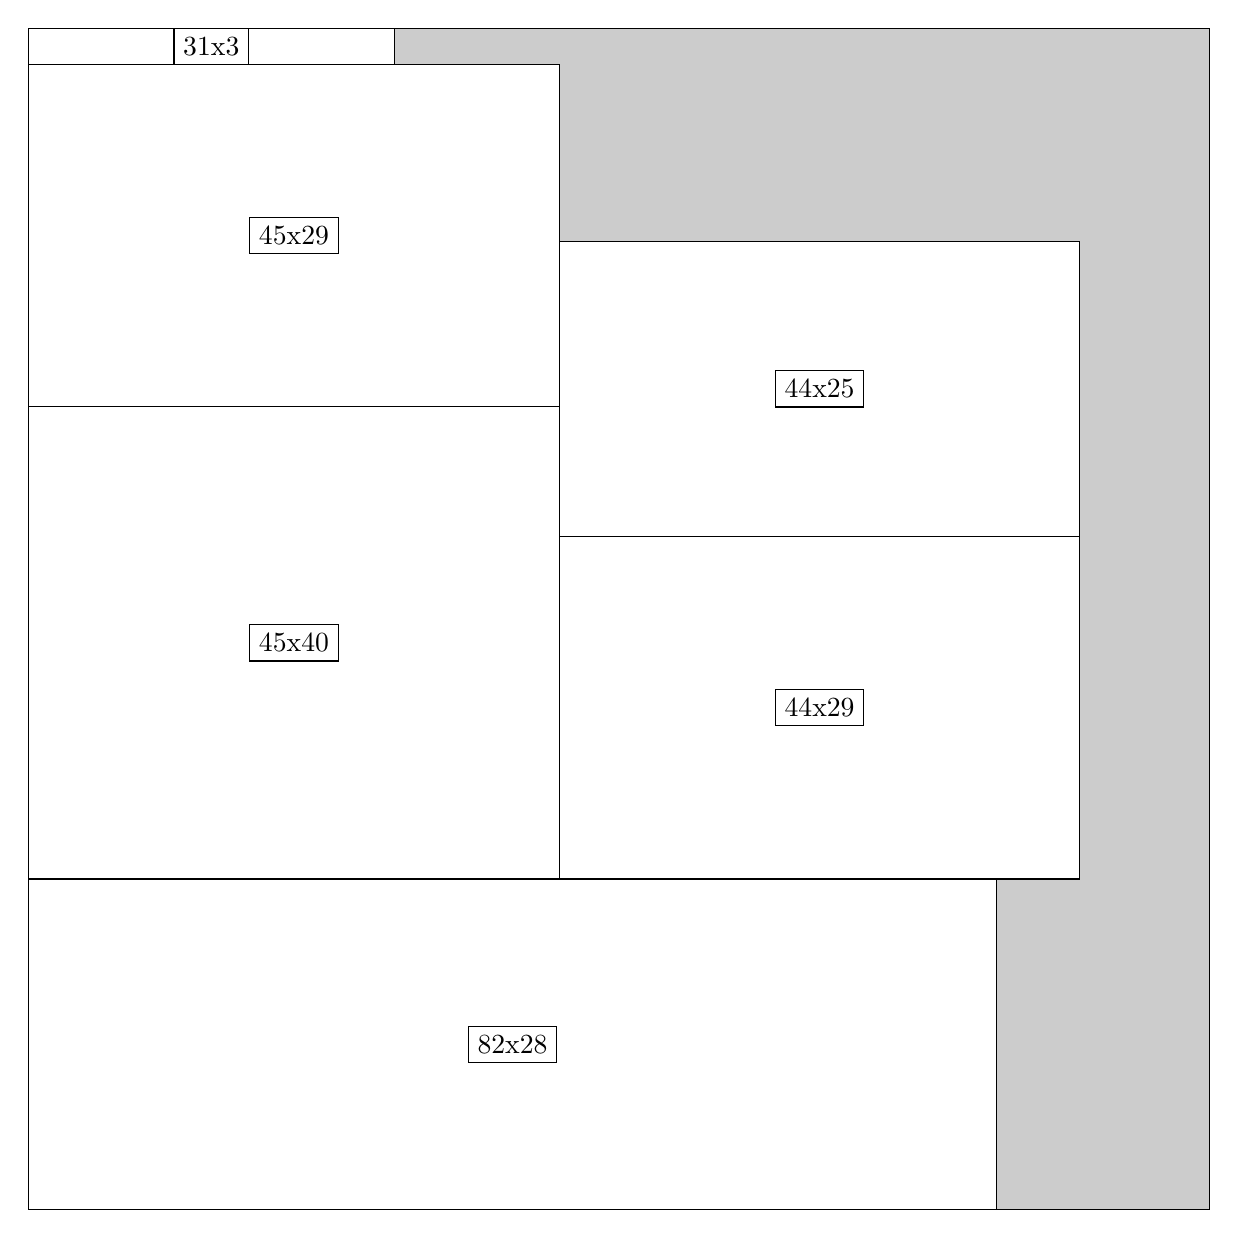
\begin{tikzpicture}[shorten >=1pt,scale=1.0,every node/.style={scale=1.0},->]
\tikzstyle{vertex}=[circle,fill=black!25,minimum size=14pt,inner sep=0pt]
\filldraw[fill=gray!40!white, draw=black] (0,0) rectangle (15.0,15.0);
\foreach \name/\x/\y/\w/\h in {82x28/0.0/0.0/12.299999999999999/4.2,45x40/0.0/4.2/6.75/6.0,45x29/0.0/10.2/6.75/4.35,44x29/6.75/4.2/6.6/4.35,44x25/6.75/8.549999999999999/6.6/3.75,31x3/0.0/14.549999999999999/4.6499999999999995/0.44999999999999996}
\filldraw[fill=white!40!white, draw=black] (\x,\y) rectangle node[draw] (\name) {\name} ++(\w,\h);
\end{tikzpicture}


w =82 , h =28 , x =0 , y =0 , v =2296
\par
w =45 , h =40 , x =0 , y =28 , v =1800
\par
w =45 , h =29 , x =0 , y =68 , v =1305
\par
w =44 , h =29 , x =45 , y =28 , v =1276
\par
w =44 , h =25 , x =45 , y =57 , v =1100
\par
w =31 , h =3 , x =0 , y =97 , v =93
\par
\newpage


\end{document}